\chapter{Vývojová dokumentace knihovny GTTG}
Ve Visual Studio 2017 \textit{solution} se nachází celý obsah práce, kde knihovna GTTG je jednou z~jeho částí.
Představíme si, jak je celý solution strukturovaný a~jaké jsou jeho další části. Solution jsme rozdělili
do tří složek:
\newline
\newline
\renewcommand\arraystretch{1.2}
\begin{tabular}{ m{0.1\textwidth} m{0.84\textwidth} }
\texttt{build} & Společná nastavení verzí balíčků používána v~projektech. Na soubory v~\texttt{build} typu \textit{*.props} obsahující verze balíčků se odkazují projekty v~\textit{.csproj} souborech.\\
\texttt{src} & Zdrojový kód v~solution\\ 
\texttt{test} & Unit testy pro zdrojový kód v~\texttt{src}
\end{tabular}
\newline
\newline
Solution je rozděleno do sedmi projektů uvedených na obrázku \ref{fig:kap4:solution_structure}, představující dvě části -- knihovnu GTTG, jejímuž popisu jsme se doposud věnovali, a~aplikaci SZDC, implementující práci s~grafikonem vlakovy využitím knihovny podle cíle \textbf{\ref{uvod:cil:aplikace}}. Popisu aplikace se budeme věnovat v~kapitole \ref{kap6:szdc_app}.

\begin{figure}[!hbt]
	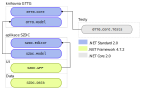
\includegraphics[width=\textwidth]{../img/kap4_solution_structure}
	\caption{Struktura projektů v~solution}
	\label{fig:kap4:solution_structure}
\end{figure}

Podle cíle~\textbf{\color{goalcolor}G2}\ref{uvod:cil:knihovna:dotnet_standard} jsme pro co největší přenositelnost knihovny GTTG všechny její projekty  implementovali vůči rozhraní .NET Standard 2.0. Jelikož podle cíle \textbf{\color{goalcolor}G2}\ref{uvod:cil:aplikace:vice_gui} chceme logiku aplikace SZDC zapojit do více uživatelských rozhraní, je také její editor \texttt{SZDC.Editor} a~model dat \texttt{SZDC.Model} implementován vůči rozhraní .NET Standard. Jako GUI framework aplikace \texttt{SZDC} jsme zvolili WPF, který je v~naší aplikaci spustitelný na běhovém prostředí .NET Framework 4.7.2. Nově je možné i WPF spustit na běhovém prostředí .NET Core 3. Výběru GUI frameworku a~běhového prostředí pro zvolené WPF se věnujeme v~kapitole \ref{kap6:szdc_gui_framework}.

\subsubsection*{Struktura knihovny GTTG}
Knihovna je rozdělena do dvou spolu souvisejících částí, jejichž schéma rozdělení se nachází na obrázku \ref{fig:kap4:gttg_lib_structure}.

\texttt{GTTG.Core} obsahuje nástroje umožňující uživatelskou interakci s~knihovnou a~její integraci do aplikací. Základem knihovny je \textit{engine} \texttt{GraphicalComponent} a~nástroj \texttt{DrawingManager} rozdělující kreslení do vrstev. Dále jsou v~projektu implementovány prvky umožňující systematicky popsat implementaci nákresných jízdních řádů, jako třeba \texttt{ViewElement} a~\texttt{Visual}. 
Projekt obsahuje nástroje pro práci s~těmito prvky, jako třeba \texttt{HitTestManager} a~nabízí rozhraní jako \linebreak\texttt{IStrategyDocker}, jehož implementací vytváří vývojář strategie umisťující prvky jako kóty do nákresného jízdního řádu.

\texttt{GTTG.Model} používá \texttt{GTTG.Core} k~vytvoření základního modelu nákresných jízdních řádů. Třídy jako \texttt{TrainView} jsou potomky základní třídy zobrazitelných prvků \texttt{ViewElement} a~představují vizualizaci datového modelu tříd jako \texttt{Train} nebo \texttt{Station}. Projekt tak rozděluje třídy na \textit{view model} a~\textit{model}. Dále jsou v~projektu implementována rozhraní knihovny \texttt{GTTG.Core} pro práci se zobrazitelnými prvky. Například \texttt{TracksStrategyDocker} jako implementace rozhraní \texttt{IStrategyDocker} z~\texttt{GTTG.Core} rozmisťuje kóty \includegraphics[height=10.0pt]{../img/cas_osa_typ_1} do ostrých úhlů průběhu jízdy vlaku \texttt{TrainView}.

\begin{figure}[!hbt]
	\centering
	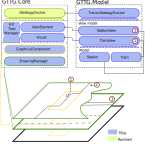
\includegraphics[width=.85\textwidth]{../img/kap4_gttg-lib-structure}
	\caption{Části knihovny GTTG}
	\label{fig:kap4:gttg_lib_structure}
\end{figure}

\section{GTTG.Core}
\texttt{GTTG.Core} \textit{assembly} je rozdělena do několika oblastí jmenných prostorů:

\begin{tabular}{ m{0.15\textwidth} m{0.70\textwidth} }
\texttt{Base} & Hierarchie tříd implementující zobrazitelné prvky \\
\texttt{Component} & Třídy pro práci s~grafickou komponentou \\ 
\texttt{Drawing} & Nástroje pro kreslení \\
\texttt{Extensions} & Knihovní a~SkiaSharp \textit{extension} metody \\
\texttt{HitTest} & Nástroje pro hit-testování obsahu \\
\texttt{Strategies} & Nástroje pro práci se strategiemi \\
\texttt{Time} & Třídy pro reprezentaci časových intervalů \\
\texttt{Utils} & Matematické funkce pro implementaci strategií
\end{tabular}
\newline
\newline
V~následujících částech si tyto jmenné prostory popíšeme.

\subsection{Grafická komponenta}
\label{kap4:graphical_component}
Základem knihovny GTTG je třída \texttt{GraphicalComponent} představující \textit{engine}, který umožňuje vytvářet pohled na nákresný jízdní řád podle interakcí uživatele s~aplikací nebo jiných nastavení, jako na obrázku \ref{fig:kap4:gttg-core-graphical-component}. Poskytuje modifikace jako translace a~škálování pohledu v~rámci ohraničení nákresného jízdního řádu. Na základě nastavení pohledu pak vzniká stav komponenty, s~kterým pracují ostatní části knihovny. Například vykreslení nákresného jízdního řádu je nastaveno maticí \texttt{ContentMatrix},  kterou podle \ref{fig:analyza_impl:platno} třída modifikacemi upravuje.

\begin{figure}[!hbt]
	
\includegraphics[width=\textwidth]{../img/kap4_gttg-core-graphical-compont}
	\caption{\textit{Engine} \texttt{GraphicalComponent}}
	\label{fig:kap4:gttg-core-graphical-component}
\end{figure}

Obrázek \ref{fig:kap4:gttg-core-component_structure_diagram} obsahuje schéma tříd jmenného prostoru \texttt{GTTG.Core.Component} související s~implementací grafické komponenty, jehož součásti si nyní blíže představíme:

\begin{figure}[!hbt]
	
\includegraphics[width=\textwidth]{../img/kap4_gttg-core-component_structure_diagram}
	\caption{Schéma tříd a~rozhraní implementujících grafickou komponentu}
	\label{fig:kap4:gttg-core-component_structure_diagram}
\end{figure}

\newpage
Stav komponenty \ref{spec:req:state} je představován vlastnostmi, které jsou mimo třídu pouze pro čtení. Abychom mohli stav v~komponentě poskytnou dalším částem knihovny nebo implementacím bez přístupu k~modifikacím komponenty, \linebreak\texttt{GraphicalComponent} implementuje rozhraní \texttt{IViewProvider}. Rozhraní poskytuje i~převody mezi body komponenty a~časovými údaji, které jsou využívány nástroji knihovny (průběh jízdy vlaku se vykreslí převodem jeho časových údajů do souřadnic) nebo naopak aplikační logikou pracující s~knihovnou, která chce souřadnice kurzoru myši v~komponentě převést na časový údaj zobrazený v~aplikaci.

Komponenta pracuje s~třídou \texttt{ViewModifier} určenou pro vykonávání složitějších matematických modifikací stavu komponenty. Implementace modifikací v~\texttt{GraphicalComponent} upraví parametry a~předá je odpovídající modifikaci ve \texttt{ViewModifier}. V~případě úspěšné modifikace je pak upraven celý stav komponenty. Každá modifikace vrací podle \ref{kap3:modifikace_komponenty} výčtový typ nesoucí informace
o~jejím výsledku.

\subsubsection*{Práce s~časovými údaji}
Knihovna obsahuje strukturu \texttt{DateTimeInterval} představující časové intervaly \texttt{DateTime} hodnot. \texttt{GraphicalComponent} tuto strukturu používá k~reprezentaci časových intervalů v~komponentě popsaných v~\ref{kap2:time_intervals}. Třídou \texttt{DateTimeContext}, která tyto intervaly slučuje a~zajišťuje jejich validitu, se můžou komponentě v~rámci jejího stavu přenastavit časové intervaly. Pohled na nákresný jízdní řád je pak možné modifikovat i~pomocí časových intervalů jako v~situacích zmíněných v~\ref{kap2:modifikace_cas_intervaly}.

\subsection{Vykreslování}
Obsah knihovny je vykreslován ve vrstvách, které jsou reprezentovány rozhraním \texttt{IDrawingLayer} s~metodou \texttt{Draw()} k~vykreslení vrstvy. Podle schématu \ref{fig:kap4:drawing_layers_diagram} abstraktní třída \texttt{DrawingLayer} implementuje toto rozhraní a~je předkem tří abstraktních typů vrstev:

\hskip-1.0cm
\begin{tabular}{ m{0.33\textwidth} m{0.63\textwidth} }
\texttt{ContentDrawingLayer} & Typ vrstvy, které je k~vykreslení poskytnuto plátno pro celý obsah nákresného jízdního řádu podle \ref{spec:req:canvas1}. \\
\texttt{ViewDrawingLayer} & Typ vrstvy, které je k~vykreslení poskytnuto plátno komponenty podle \ref{spec:req:canvas2}. \\ 
\texttt{DefaultDrawingLayer} & \textit{Singleton} reprezentující vrstvu, která je při kontrole vrstvy v~\ref{kap3:drawing_layers} vždy validní.
\end{tabular}

\begin{figure}[!hbt]
	\centering
	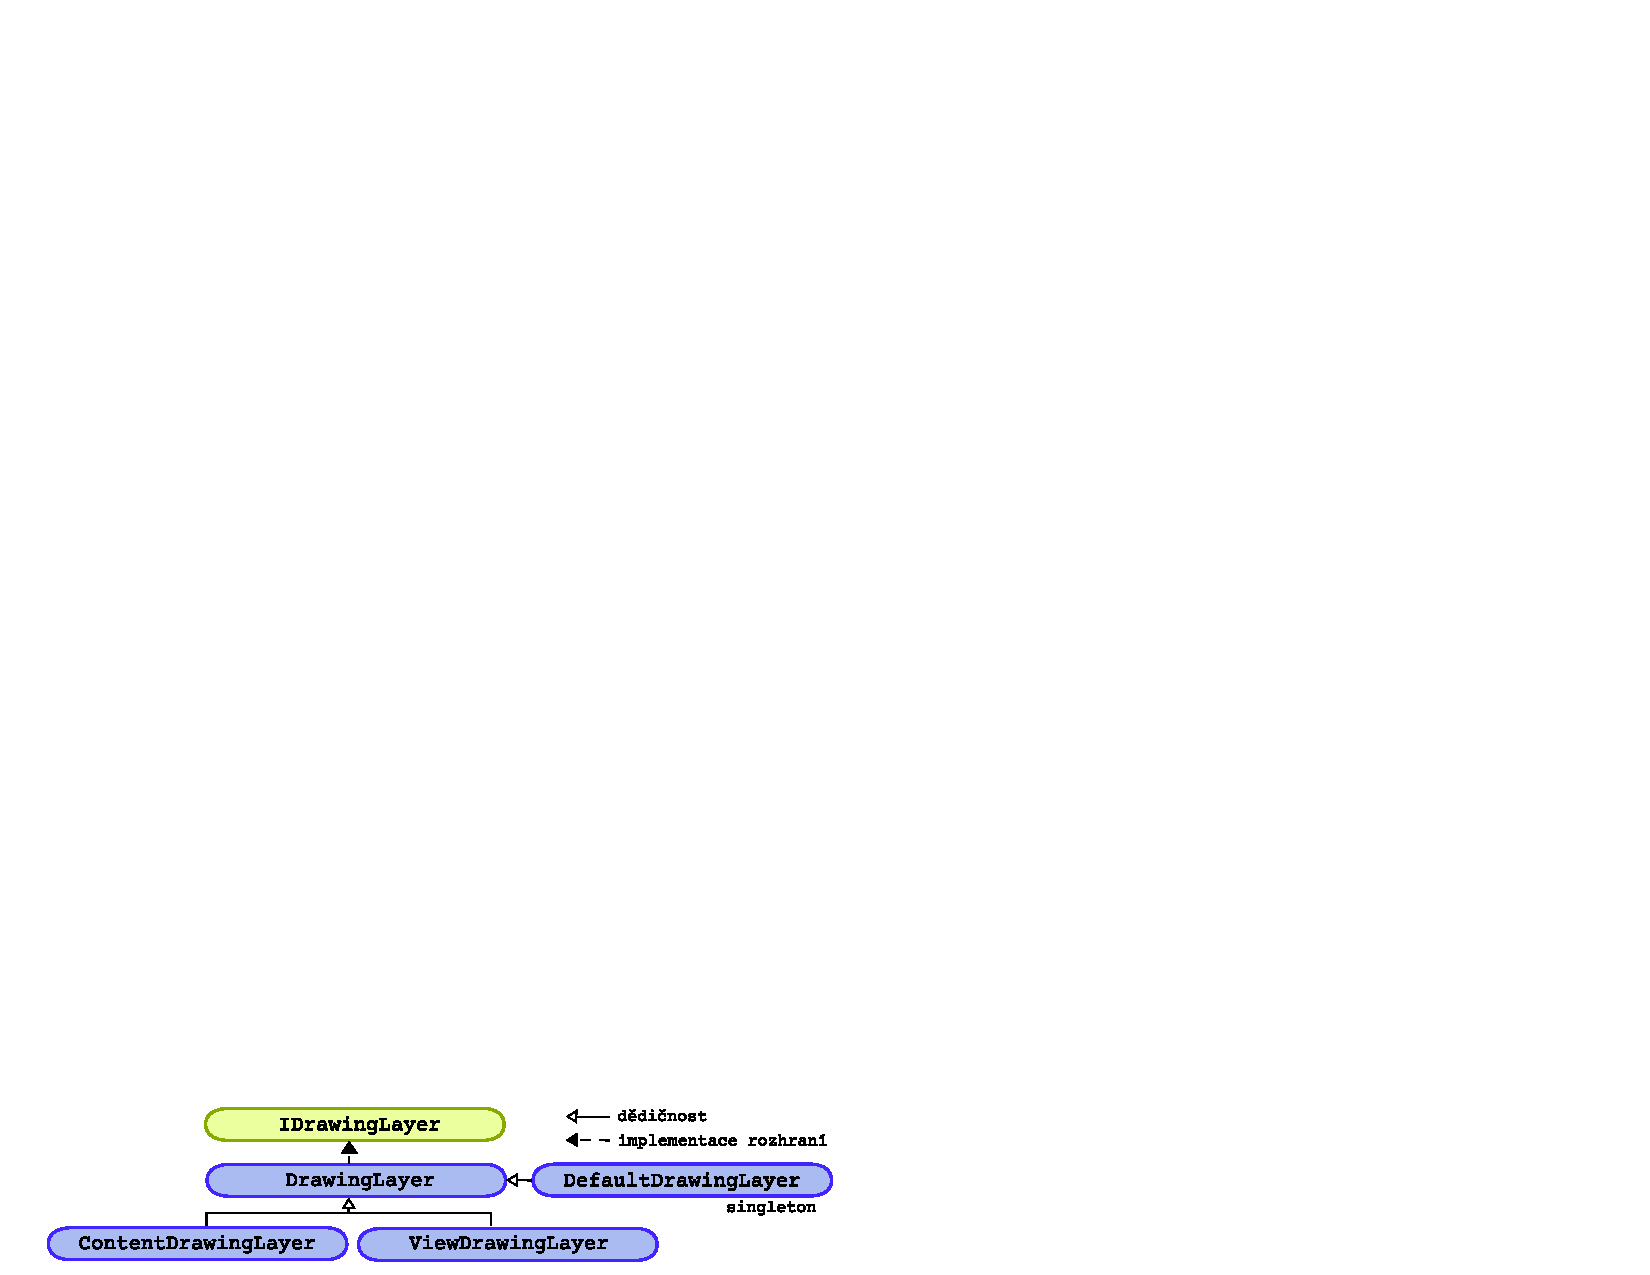
\includegraphics[width=\textwidth]{../img/kap4_gttg-core_drawing_layers1}
	\caption{Schéma tříd a~rozhraní představující vrstvy}
	\label{fig:kap4:drawing_layers_diagram}
\end{figure}

\subsubsection*{Správa kreslících vrstev}
Třída \texttt{DrawingManager} vykresluje vrstvy podle pořadí definovaného vývojářem. Instance vrstev jsou přidávány s~určením jejich pořadí pomocí metod \texttt{AddOnCurrentTop()}, \texttt{AddOnCurrentBottom()}, \texttt{Insert()}. Instanci vrstvy je \linebreak možné odstranit pomocí \texttt{RemoveDrawingLayer()}. Jelikož existují vrstvy, které se neodstraňují a~jejich pořadí je během běhu aplikace neměnné, konstruktoru \texttt{DrawingManager} se předává implementace rozhraní \texttt{IRegisteredLayersOrder}, které obsahuje pořadí typů (z~\texttt{typeof()}) vrstev, které označíme jako \textit{registrované}. Takovou vrstvou může být vrstva svislých čar reprezentující časové údaje nebo vrstva s~dopravními body. Metoda \texttt{ReplaceRegisteredDrawingLayer()} umístí instanci registrované vrstvy podle jejího  typu v~pořadí určeným~rozhraním.

\subsubsection*{Kreslící plátno}
Knihovna na plátno \texttt{SKCanvas}, které ji poskytne vývojář, vytváří různé pohledy. Tyto pohledy budeme reprezentovat plátnem \texttt{DrawingCanvas}. Vhodným nastavením \texttt{transformation matrix} na \texttt{SKCanvas} může \texttt{DrawingCanvas} představovat plátno pro vykreslování zobrazitelných prvků z~\ref{kap3:vykresleni_zobrazitelnych_prvku} i~celého obsahu plátna \texttt{ContentCanvas} z~\ref{fig:analyza_impl:platno}. Plátno nabízí kreslící příkazy \texttt{SKCanvas} a~příkazy pro vykreslení prvků knihovny. Plátno obsahuje vlastnosti o~své velikosti \texttt{Width}, \texttt{Height}. Vlastnost \texttt{DrawingLayer} udává, v~jaké vrstvě bylo plátno vytvořeno.

\subsubsection*{Proces vykreslování vrstev}
\textit{Entry pointem} pro vykreslení obsahu knihovny je metoda \texttt{Draw(SKSurface surface)} ve třídě \texttt{DrawingManager}. Vrstvy se vykreslí v~sestaveném pořadí tak, že se pro každou vrstvu zavolá metoda \texttt{CreateCanvas()} factory rozhraní \linebreak\texttt{ICanvasFactory}, která poskytnutím \texttt{IDrawingLayer} a~\texttt{SKCanvas} vytvoří pro vrstvu konfigurovaný \texttt{DrawingCanvas}. Vrstvám \texttt{ContentDrawingLayer} \linebreak a~\texttt{ViewDrawingLayer} poskytuje knihovna implementaci rozhraní \texttt{CanvasFactory}.

\begin{figure}[!hbt]
	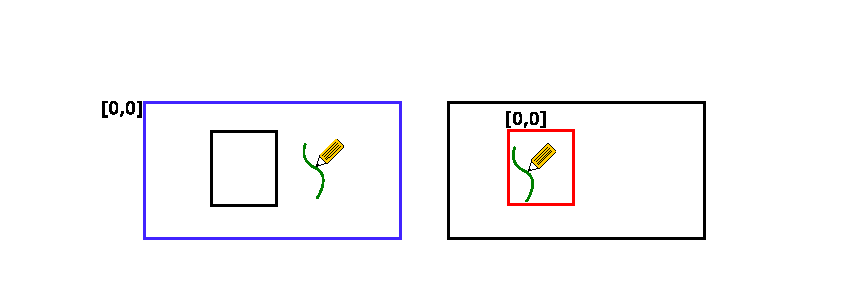
\includegraphics[width=\textwidth]{../img/kap4_gttg-core_drawing_canvases}
	\caption{Modře ohraničený \texttt{ContentDrawingCanvas} a~červeně ohraničený \texttt{ViewDrawingCanvas}}
	\label{fig:kap4:gttg-core-base_canvases}
\end{figure}

\newpage
\subsection{Zobrazitelné prvky}
Jmenný prostor \texttt{GTTG.Core.Base} obsahuje hierarchii tříd uvedenou na obrázku \ref{fig:kap4:gttg-core-base_class_hierarchy}, z~níž vzniká třída \texttt{ViewElement} představující zobrazitelné prvky určené k~systematickému popisu nákresného jízdního řádu podle \ref{kap2:view_elements}.

\begin{figure}[!hbt]
	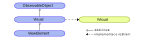
\includegraphics[width=\textwidth]{../img/kap4_gttg-core-base_class_hierarchy}
	\caption{Hierarchie tříd tvořící zobrazitelné prvky}
	\label{fig:kap4:gttg-core-base_class_hierarchy}
\end{figure}

\subsubsection*{ObservableObject}
\label{kap4:observable_object}
Na začátku hierarchie tříd se nachází abstraktní třída \texttt{ObservableObject} implementující rozhraní \texttt{INotifyPropertyChanged}, které slouží k~notifikacím o~změnách vlastností v~třídě pomocí eventu \texttt{PropertyChanged}. Tuto základní třídu mohou využít vývojáři k~vytvoření \textit{data bindingu} z~uživatelských rozhraní na aplikační logiku a~její model. Pokud bychom měli například model vlaku \texttt{Train} obsahující plán jízdy \texttt{Schedule}, aplikace by \texttt{Schedule} navíc zobrazovala v~jiné komponentě uživatelského rozhraní jako textová data. V~případě, kdy by se \texttt{Schedule} změnila, notifikaci o~změně obdrží jiná komponenta v~aplikaci a~zároveň i~\texttt{TrainView}, které může upravit svou vizualizaci dat. Z~této třídy dědí \texttt{GraphicalComponent}, která tak umožňuje vývojářům získávat notifikace o~změně \texttt{DateTimeContext}. 

Třída implementuje mechanismus pro bezpečné a~lehké používání notifikací na \textit{setterech} vlastností, který jsme převzali z~projektu \texttt{Core2D}~\cite{Core2D} z~třídy \linebreak\texttt{ObservableObject}. Následující fragment kódu ukazuje přiřazení nové hodnoty do vlastnosti s~notifikováním pomocí \texttt{Update()} metody. Update by se jinak musel provádět pomocí \textit{invoke} eventu \texttt{PropertyChanged} poskytnutím jména vlastnosti.

\begin{csharpcode}
public class GraphicalComponent {
	
	public DateTimeContext DateTimeContext  {
		get => _dateTimeContext;
		protected set => Update(ref _dateTimeContext, value);	
	}
	
\end{csharpcode}
\newpage
\subsubsection*{Visual}
Abstraktní třída \texttt{Visual} představuje prvky, které popisují nákresný jízdní řád a~je možné je vykreslit na \texttt{DrawingCanvas}, ale narozdíl od zobrazitelných prvků se nerozmisťují. Příkladem může být prvek \texttt{TrafficView}, který sdružuje a~vykresluje na plátno \texttt{ContentDrawingCanvas} všechny vlaky \texttt{TrainView}. \texttt{Visual} obsahuje podle \ref{kap3:drawing_layers} zásobník vrstev \texttt{IDrawingLayer} s~neměnným spodkem obsahující singleton \texttt{DefaultDrawingLayer}. Vlastnost \texttt{CurrentDrawingLayer} odpovídá vrchu zásobníku. Vykreslení probíhá tak, že se virtuální metodě \texttt{Draw()} předá \texttt{DrawingCanvas} a~nejdříve se ověří možnost prvek vykreslit pomocí \linebreak \texttt{IsInDrawingLayer()} porovnáním \texttt{CurrentDrawingLayer} a~\texttt{DrawingLayer} \linebreak plátna. Po ověření se zavolá virtuální \texttt{protected OnDraw()} k~vykreslení implementace prvku.

Vyvojáři implementují \texttt{protected} \texttt{ProvideVisuals()}, která dodává prvky v~pořadí vykreslení. Metoda je volána \texttt{ProvideVisualsInSameLayer()} poskytující pouze z~těchto prvků ty, které se nachází ve stejné vrstvě jako prvek, na kterém se metoda volá. Tyto metody se používají při hit-testování a~nastavování vrstev potomkům.

Pro případy, kdy existující prvek (například model jako potomek jiné třídy) nemůže již od \texttt{Visual} dědit a~přesto chce kreslit na plátno, použije rozhraní \texttt{IVisual}, s~kterým pak pracuje i~kód knihovny jako s~reprezentací \texttt{Visual}. Rozhraní se používá i~pro \textit{mockování} v~unit testech.

\subsubsection*{ViewElement}
Abstraktní třída \texttt{ViewElement} představuje základní implementaci zobrazitelných prvků z~podkapitoly \ref{kap3:zobrazitelne_prvky}, které je možné umístit a~určit jim velikost. Pro implementaci cyklu rozmístění \texttt{ViewElement} jsme použili cyklus rozmístění prvků uživatelského rozhraní GUI frameworku WPF. Implementace jeho metod na schématu \ref{fig:arrange_WPF_kap4} odpovídá zdrojovému kódu metod z~WPF, který byl ale upraven, aby mohl vytvářet během cyklu rozmístění i~struktury, s~kterými pracuje knihovna.

\begin{figure}[!bht]
	\centering
	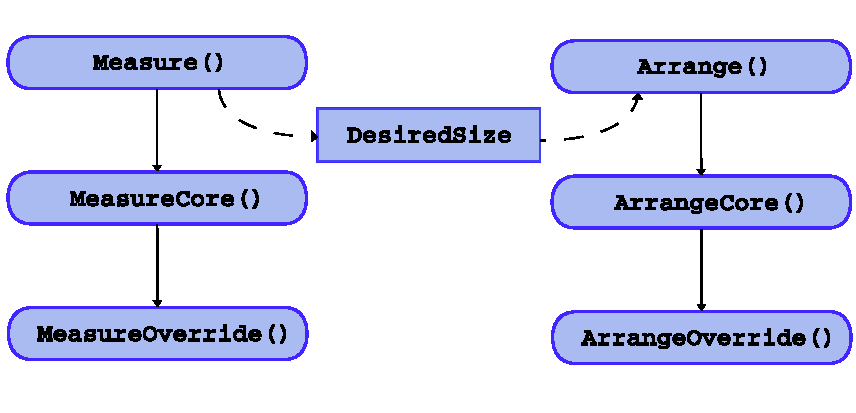
\includegraphics[width=\textwidth]{../img/kap3_wpf_element_layout_cycle_diagram}
	\caption{Schéma cyklu rozmístění pro prvek GUI frameworku WPF}
	\label{fig:arrange_WPF_kap4}
\end{figure}

\newpage
Metody \texttt{Arrange()} a~\texttt{Measure()} zajišťují správné používání virtuálních metod typu \texttt{Core}, které volají. Ty slouží k~určení obecné implementace prvků, která se používá v~rámci nějaké aplikace. V~základní implementaci upravují vrácené hodnoty z~\texttt{Override} metod. Ty jsou určeny ke změření a~rozmístění konkrétního prvku. V~rámci volání metody \texttt{Arrange()} se podle \ref{kap3:zobrazitelne_prvky} vytváří struktury, s~kterými knihovna pracuje:

\hskip-1.0cm\renewcommand\arraystretch{1.5}
\begin{tabular}{ m{0.3\textwidth} m{0.65\textwidth} }
\texttt{BoundingRectangle} & Obdélník k~určení, zda se prvek nachází v~komponentě podle \ref{fig:analyza_impl:platno}. \\
\texttt{PlacementMatrix} & Matice \texttt{placement matrix} pro vytvoření \texttt{transform matrix} plátna \texttt{DrawingCanvas} z~\ref{kap3:vykresleni_zobrazitelnych_prvku}. \\
\texttt{Clip} & Oblast ořezu vykreslení z~\ref{kap3:skia_intro_transformations} pokrývající prvek, která se může aplikovat pomocí vlastnosti \texttt{HasClipEnabled}. \\ 
\end{tabular}
\newline
\newline
Přetíženou metodou \texttt{Arrange()} se prvek umístí na plátno \texttt{ContentCanvas} -- přímo v~jeho souřadnicích nebo v~souřadnicích již umístěného prvku, který se uvede jako parametr \texttt{Arrange()} metody. To je užitečné v~případě, kdy \linebreak v~\texttt{ArrangeOverride()} rodičovského prvku získáme konečnou velikost rodiče \linebreak a~musíme v~rámci této velikosti rozmístit jeho potomky \texttt{Arrange()} metodou. Zároveň \texttt{ViewElement} implementuje metody \texttt{Reposition()}, \texttt{Scale()} a~\texttt{Rotate()}, které jsou používány strategiemi. Transformované zobrazení prvku je popsáno vlastnostmi, které jsou zobrazeny na obrázku \ref{fig:kap4:gttg-view-element-properties}. Vlastnosti s~prefixem \texttt{Content} odpovídají transformované velikosti a~umístění. Vlastnost umístění jako \linebreak\texttt{ContentRightTop} odpovídá umístění netransformovaného horního pravého vrcholu po aplikování transformace.

\begin{figure}[!hbt]
	\centering
	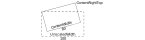
\includegraphics[width=\textwidth]{../img/kap4_gtttg-core-element-transform-properties}
	\caption{Popis vlastností \texttt{ViewElement}}
	\label{fig:kap4:gttg-view-element-properties}
\end{figure}

\subsection{Průchod stromu prvků pro hit-testování}
Průchod stromu prvků \texttt{Visual} hit-testováním popsaný v~\ref{kap3:hit_test_tree} je implementován třídou \texttt{HitTestManager} v~přetížených metodách \texttt{HitTest()}. Průchod stromem je implementován podle implementace GUI frameworku WPF -- vývojář poskytuje metody delegátů \texttt{HitTestResultCallback} a~
\texttt{HitTestFilterCallback} pro řízení průchodu stromem a~získání úspěšně otestovaných prvků, více popsané v~\ref{kap3:hit_test_tree}. Vývojáři jsou dostupná přetížení metody \texttt{HitTest()}, která se svým chováním liší. Prvky jsou pokaždé poskytovány v~pořadí jejich vykreslení. První přetížení s~parametry dvou zmíněných delegátů prochází celý obsah nákresného jízdního řádu po vrstvách, kdy z~každého prvku \texttt{Visual} navštíví potomky pouze ve stejné vrstvě pomocí \texttt{ProvideVisualsInSameLayer()}. \texttt{HitTestManager} obdrží pořadí vrstev v~konstruktoru z~\texttt{DrawingManager}.
Druhému přetížení se dodává navíc prvek \texttt{Visual} a~při průchodu se získávají potomci z~\texttt{ProvideVisuals()}, poskytující prvky i~v~jiných vrstvách. Seznam prvků \texttt{Visual}, které uspěly v~hit-testu, je pak možné seřadit pomocí \textit{extension} metody \texttt{OrderByLayers()} podle pořadí vrstev. Druhé přetížení je určeno pro případy, kdy vývojář testuje obsah umístěný původně v~jedné vrstvě a~je možné, že jeho část je nyní součástí jiné vrstvy, například při testování seznamu vlaků, kdy vlaky můžou být rozděleny do více vrstev podle jejich zařazení a~nechceme procházet celý vykreslovaný obsah. Předpokládá se, že při průchodu podstromu poskytnutého prvku se navštíví všechny prvky pouze jednou.

\subsection{Nástroje pro strategie}
V~této části si představíme implementaci nástrojů pro práci se strategiemi, které jsme si popsali v~\ref{kap2:strategies_introduction}. Na obrázku \ref{fig:kap4:gttg-strategy_tools_schema} se nachází závislosti mezi těmito nástroji. Instance třídy \texttt{Segment} představují pruhy, jejichž umístěním a~velikostí vývojář určuje místa, do kterých mají strategie rozmisťovat prvky. Přidání prvků do strategie probíhá ve třídě \texttt{StrategyManager}, která podle informací dodaných při přidávání prvku daný prvek zařadí do vhodného segmentu. Během cyklu rozmístění pak \texttt{IStrategyDocker} představující implementaci strategie obdrží všechny přidané prvky a~umístí je do segmentů podle pravidel strategie.

\begin{figure}[!hbt]
	\centering	
	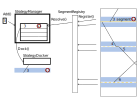
\includegraphics[width=0.8\textwidth]{../img/kap4_gtttg-core-strategies-tools}
	\caption{Schéma nástrojů pro práci se strategiemi}
	\label{fig:kap4:gttg-strategy_tools_schema}
\end{figure}

\subsubsection*{Segmenty}
\label{kap4:segments}
Třída \texttt{Segment} představuje podle \ref{kap3:implementace} ohraničený horizontální pruh, kterému se určuje výška. Podle výšky segmentu se do něj strategiemi rozmisťují prvky. Pokud je segment pro prvek příliš krátký, může strategie podle \ref{kap2:strategies_introduction} prvek zmenšit škálováním. Výška segmentu se určuje v~rámci \texttt{ArrangeOverride()} nějakého zobrazitelného prvku. Například prvek \texttt{StrategyStationView} obsahuje segmenty, které se umisťují kolem horizontálních čar představující koleje k~rozmístění údajů do ostrých úhlů. Segmentům se přiřadí ohraničení a~velikost pomocí přetížených metod \texttt{SetBounds()}. Pokud vývojář chce určit výšku segmentu na základě prvků, které jsou do něj přidány, použije potomka \texttt{MeasurableSegment}, který výšku měří hledáním maxima voláním eventu, do nějž se přidají měření výšek jednotlivých prvků v~segmentu.

Instance segmentů je možné registrovat v~třídě \texttt{SegmentRegistry}, do které se segmenty přidávají pod typovým argumentem \texttt{TSegmentType}, zvoleným při vytváření \texttt{SegmentRegistry}. Pomocí \texttt{TSegmentType}, který může být například strukturou obsahující přesné informace o umístění segmentu, pak můžou ostatní části knihovny získávat ze \texttt{SegmentRegistry} konkrétní registrované instance. Dále \texttt{SegmentRegistry} umožňuje pomocí \textit{fluent syntax} registrovat jednu instanci segmentu pod více \texttt{TSegmentType} argumenty, jako na následujícím fragmentu kódu:

\begin{csharpcode}
 var segmentType1 = /*...*/;
 var segmentType2 = /*...*/;
 var segment = /*...*/;
 segmentRegistry.Register(segment).As(segmentType1).As(segmentType2);
\end{csharpcode}

Rozhraní \texttt{ISegment} slouží pro přístup ke čtení vlastností segmentu mimo prvek, který ho rozmisťuje.

\subsubsection*{StrategyManager}
\label{kap4:strategy_manager}
Vývojář přidává prvky do segmentů k~aplikování strategií pomocí třídy \linebreak\texttt{StrategyManager}, která je určena 4 typovými argumenty:\newline

\hskip-1.0cm\renewcommand\arraystretch{1.5}
\begin{tabular}{ m{0.25\textwidth} m{0.65\textwidth} }
\texttt{TPlacementType} & Typ, kterým vývojář určí, kam se prvek umístí \\ 
\texttt{TElement} & Typ přidávaného prvku, který je potomkem \texttt{IVisual} \\
\texttt{TSegmentType} & Typ používaný ke kategorizaci segmentů \\
\texttt{TSegment} & Typ segmentu \\
\end{tabular}
\newline
\newline
S~\texttt{TPlacementType} pracuje \texttt{StrategyManager} jako s~klíčem, pod nímž nemůže být přidáno více prvků. Pokud bychom chtěli podle \ref{kap4:strategy_placement_type} přidat odjezdovou kótu do segmentu koleje, \texttt{PlacementType} bude obsahovat výčtový typ s~hodnotami \texttt{Departure} / \texttt{Arrival}, udávájící umístění v kontextu průběhu jízdy vlaku. \texttt{StrategyManager} převede pomocí implementace převodů \texttt{ITypeConverter} (dodané v konstruktoru) tento typ na \texttt{TSegmentType}, který je strukturou s výčtovým typem s identifikátorem stanice a hodnotami \texttt{Upper} / \texttt{Lower}, udávající umístění segmentu nad nebo pod horizontální čarou stanice. Celý průběh přidání prvku je pak následující:

\begin{enumerate}
\item  Klíč \texttt{TPlacementType} se pomocí \texttt{ITypeConverter} převede \newline na \texttt{TSegmentType}
\item  Pomocí \texttt{TSegmentType} se získá ze \texttt{SegmentRegistry} instance segmentu
\item  Do \texttt{StrategyManager} se uloží přidávaný prvek, typ umístění i~typ segmentu a~segment, který se prvku přiřadil. Ty jsou pak přístupné implementacím \texttt{IStrategyDocker}.
\end{enumerate}

\texttt{MeasureableStrategyManager} jako rozšíření této třídy v~konstrukturu přijímá rozhraní \texttt{IElementMeasureProvider} sloužící ke změření výšky přidávaného prvku do segmentu \texttt{MeasureSegment}. Pokud vývojář nepotřebuje pracovat s~instancemi segmentů a~\texttt{SegmentRegistry}, může využít  \texttt{BasicStrategyManager}, která je předkem \texttt{StrategyManager} a~pouze pracuje s~\texttt{TPlacementType} \linebreak a~\texttt{TSegmentType}.

\subsubsection*{IStrategyDocker}
Dockery strategií jako implementace rozhraní \texttt{IStrategyDocker} rozmisťují prvky do segmentů aplikováním různých strategií, uvedených v~\ref{kap2:strategies_introduction}. Rozhraní \texttt{IStrategyDocker} obsahuje pouze metodu \texttt{Dock()}, která je volána v~cyklu rozmístění.
Metoda rozmístí prvky, které získá v~konstruktoru, nejčastěji třídu \linebreak \texttt{StrategyManager}. Jelikož docker prvky rozmisťuje, může také určovat jejich výšku v~segmentu -- proto může implementovat \texttt{IElementMeasureProvider}. \linebreak \texttt{StrategyManager}, jehož prvky docker umisťuje, poskytuje ke~každému prvku jeho segment a~další ukládané informace, na jejichž základě je docker schopný určit přesné umístění prvku pomocí vyměřování matematickými funkcemi z~jmenného prostoru \texttt{GTTG.Core.PlacementUtils}.

\newpage
\section{Pokrytí požadavků unit testy}
\label{kap4:requirements_coverage}
\newcommand{\comp}[0]{\textbf{\color{red}COMP}}
\newcommand{\dti}[0]{\textbf{\color{blue}DTI}}
\newcommand{\ve}[0]{\textbf{\color{green}VE}}
\newcommand{\dl}[0]{\textbf{\color{orange}DL}}
\newcommand{\hit}[0]{\textbf{\color{purple}HT}}

Unit testy jsou implementovány v~projektu \texttt{GTTG.Core.Tests} vůči běhovému prostředí \texttt{.NET Core} 2.0. K~implementaci testů jsme použili unit test framework xUnit~\cite{xUnit} a~\textit{mock} knihovnu Moq~\cite{moq}. V~následující tabulce se nachází oblasti požadavků, které jsme v~testech pokryli. Každý test má pomocí atributu přidělené číslo požadavku v~projektu testů, skládající se ze zkratky oblasti požadavků a~unikátního čísla v~této oblasti (neodpovídající očíslování požadavků v~textu), jako na následujícím fragmentu kódu:

\begin{csharpcode}
[Trait("Req.no", "COMP16")]
public void TranslateScaleOutOfBounds() { /*...*/ }
\end{csharpcode}

\subsubsection*{Rozdělení do oblastí požadavků}
\hskip-0.5cm\begin{tabular}{ | m{5cm} | m{4cm} | m{3.5cm} | }
\hline
\textbf{Oblasti požadavků} & \textbf{Rozsah požadavků} & \textbf{Tag pro unit test} \\
Modifikace komponenty  &  \ref{spec:req:interaction_trans1} - \ref{spec:req:interaction_zoom2} & \comp \\
Práce s~čas. intervaly & \ref{spec:req:int1} - \ref{spec:req:width_mod1}, \ref{spec:req:time_mod1}-\ref{spec:req:time_mod3} & \dti \\
Zobrazitelné prvky & \ref{spec:zobrazitelne_prvky1} - \ref{spec:zobrazitelne_prvky2} & \ve \\
Vrstvy kreslení & \ref{spec:req:layers1} - \ref{spec:req:layers3} & \dl \\
Hit-testování & \ref{spec:req:hit-test1} - \ref{spec:req:hit-test2} & \hit \\
\hline
\end{tabular}
\newline
\newline
V~další tabulce jsou uvedena přímá pokrytí požadavků konkrétními testy.

\subsubsection*{Přímé pokrytí}
\hskip-0.5cm\begin{tabular}{ | m{1cm} | m{3cm} | m{1cm} | m{3cm} | }
\hline
\ref{spec:req:interaction_trans1} & \comp 12-16 & \ref{spec:req:interaction_trans2} & \comp 7-10 \\
\ref{spec:req:interaction_zoom1} & \comp 6,11 & \ref{spec:req:interaction_zoom2} & \comp 16 \\
\ref{spec:req:int1} & \dti 10-12 & \ref{spec:req:int2} & \dti 14 \\
\ref{spec:req:width_mod1} & \comp 16 & \ref{spec:req:time_mod1} & \dti 10 \\
\ref{spec:req:layers3} & \dl 1-6 & \ref{spec:req:layers2} & \dl 7,8 \\
\ref{spec:zobrazitelne_prvky2} & \ve 11-20 & \ref{spec:req:strategie2} & \ve 1-10 \\
\ref{spec:req:hit-test2} & \hit 1-15 & & \\
\hline
\end{tabular}

\newpage
\section{GTTG.Model}
\label{kap4:model}
\texttt{GTTG.Model} \textit{assembly} obsahuje implementaci základního modelu obsahu nákresného jízdního řádu, kterou můžou aplikace používající knihovnu dále rozšiřovat, podle \ref{kap2:req:model_impl}. Implementace je v~projektu rozdělena do dvou jmenných prostorů:

\begin{tabular}{ m{0.15\textwidth} m{0.73\textwidth} }
\texttt{Model} & Třídy obsahující datovou reprezentaci modelu \\
\texttt{ViewModel} & Třídy vytvářející vizuální reprezentaci modelu v~knihovně \\ 
\end{tabular}
\newline
\newline
Model se v~rámci obou těchto reprezentací rozděluje do následujících částí:

\begin{tabular}{ m{0.25\textwidth} m{0.60\textwidth} }
\texttt{Infrastructure} & Model traťového úseku s~dopravními body \\
\texttt{Traffic} & Model vlaků v~traťovém úseku \\ 
\end{tabular}

\subsection{Model}
Knihovna vytváří nejmenší možnou základní implementaci modelu dat popisující obsah nákresných jízdních řádů. Všechny třídy modelu jsou potomky třídy \linebreak \texttt{ObservableObject} z~\ref{kap4:observable_object}, pomocí které je možné vytvářet na model data binding. 
Na obrázku \ref{fig:kap4:gttg-core-base-diagram} se nachází schéma tříd modelu. Nejdříve si popíšeme třídy v~levém sloupci vytvářející model infrastruktury traťového úseku.

\begin{figure}[!hbt]
	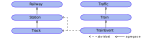
\includegraphics[width=\textwidth]{../img/kap4_gttg-core-model-diagram}
	\caption{Schéma tříd vytvářejících model}
	\label{fig:kap4:gttg-core-base-diagram}
\end{figure}

\subsubsection*{Model infrastruktury}
Třída \texttt{Railway} představuje traťový úsek obsahující kolekci tříd \texttt{Station} odpovídající dopravním bodům. Každá \texttt{Station} obsahuje koleje reprezentované třídou \texttt{Track}.

\subsubsection*{Model provozu na trati}
Třída \texttt{Traffic} seskupuje všechny vlaky. Vlaky jsou reprezentovány třídou \texttt{Train} a~obsahují plán jízdy, který se skládá z~immutable událostí \texttt{TrainEvent}. Události jsou popsány \texttt{DateTime}, \texttt{Station} a~\texttt{Track} -- odpovídají tak nějakému dopravnímu bodu na trati v~čase. Navíc obsahují vlastnost výčtového typu \linebreak\texttt{TrainEventType}, který udává informaci, zda je událost příjezdem, odjezdem nebo průjezdem.

\subsection{View modely}
View model i~model představuje stromovou strukturu tříd, které jsou na sobě závislé. Na následujícím fragmentu kódu se nachází view model pro \texttt{Station} obsahující view modely kolejí \texttt{Track}. U~modelu jako je \texttt{Station} máme k~dispozici pouze základní třídy, které je možné \textit{downcasty} přetypovat na konkrétní implementaci. Instance modelu se v~základních třídách view modelu vyskytují jako vlastnosti. Aby nebylo nutné provádět downcasty mezi třídami view modelu, v~kterých se musí často pracovat s~konkrétní implementací, jsou třídě dodány typové argumenty určující konkrétní implementaci. Na fragmentu kódu je dodán \texttt{StationView} typový argument  \texttt{TTrackView} jako konkrétní implementace \texttt{TrackView}. V~konkrétní implementaci \texttt{StationView} je možné přistoupit k~poli konkrétní implementace \texttt{TrackView} bez downcastů.

\begin{csharpcode}
public class StationView<TTrackView> : InfrastructureViewElement 
   where TTrackView : TrackView {

	public Station Station { get; }
	public ImmutableArray<TTrackView> TrackViews { get; }
\end{csharpcode}

Knihovna nekontroluje jakoukoliv logickou správnost (\textit{sanity}) dat dodaných modelem. V~případě existujících dat, které mají špatné hodnoty, komponenta vykresluje obsah špatným způsobem.

\subsubsection*{Factory metody pro tvorbu view modelu}
\label{kap4:view_model_factory_impl}
Aby bylo možné vytvořit view model přímo v~konstruktorech, vytvořili jsme rozhraní s~\textit{factory} metodami, které vytváří z~instancí modelu view model. Na následujícím fragmentu kódu se nachází rozhraní pro vytvoření konkrétní třídy \texttt{TTrackView} jako potomka \texttt{TrackView} z~modelu \texttt{Track}. View model \texttt{StationView} pak vytváří pomocí factory metod seznam konkrétních \texttt{TTrackView}. Pomocí rozhraní je tak možné nad rámec základní implementace vytvořit konkrétní třídy, kterým je možné dodat další parametry.

\begin{csharpcode}
public interface ITrackViewFactory<out TTrackView>
   where TTrackView : TrackView {
	
	TTrackView CreateTrackView(Track track);
}

public class StationView<TTrackView> : InfrastructureViewElement 
   where TTrackView : TrackView {
		
    public StationView(Station station,
                       ITrackViewFactory<TTrackView> trackViewFactory) {

		Station = station;
		TrackViews = ImmutableArray
		.CreateRange(station.Tracks.Select(trackViewFactory.CreateTrackView));
    }
}
\end{csharpcode}

\newpage
Základní implementace poskytuje dvě verze view modelu. Pro jednoduchost zavedeme [*] jako zkratku za název entity modelu, například \uv{Train}:

\begin{tabular}{ m{0.25\textwidth} m{0.60\textwidth} }
\texttt{[*]View} & Verze bez podpory strategií \\
\texttt{Strategy[*]View} & Třídy obsahující prefix \textit{Strategy} implementují práci se strategiemi \\ 
\end{tabular}

\subsubsection*{View model infrastruktury bez podpory strategií}
Základní view model infrastruktury pracuje se základním modelem, který jsme si představili. Neobsahuje tedy údaje kilometrické polohy dopravních bodů na trati. Prvky ve view modelu se proto rozmisťují na vertikální ose rovnoměrně. \texttt{RailwayView} obsahuje kolekci \texttt{StationView}, která obsahuje horizontální čáry kolejí \texttt{TrackView}. Pro všechny části view modelu infrastruktury platí, že v~případě, kdy výška v~\texttt{DesiredSize} přesahuje konečnou velikost přidělenou v~metodě \texttt{Arrange()}, je obsah proporčně zmenšen podobně jako v~\ref{spec:req:height_mod1}.

\subsubsection*{TrackView a~práce s~čarami}
\label{kap4:track_view_with_line_paint}
Společným prvkem implementace view modelu se strategiemi i~bez strategií je \texttt{TrackView}, který představuje oblast pro vykreslení horizontální čáry koleje \texttt{Track}. Jeho implementace zajišťuje správné umístění šikmých čar představující průběh jízdy vlaků i~horizontální čáry dopravního bodu (koleje) do horizontálního pruhu, který je  \texttt{TrackView} v~cyklu rozmístění vyhrazen. Na obrázku \ref{fig:kap4:gttg-model-track-segments} se nachází problém, který implementace odstraňuje. Když má vlak v~nějakém dopravním bodu delší dobu pobytu, jeho čára má být vykreslena na prostředek čáry v~\texttt{TrackView}. Jelikož čáry můžou mít obecně různou tloušťku, mohl by nastat problém, kdy se budou čáry překrývat se segmenty, které \texttt{StrategyStationView} kolem \texttt{TrackView} rozmisťuje. Problém se řeší v~\texttt{TrackView} pomocí segmentů, jako na obrázku \ref{fig:kap4:gttg-model-track-segments-solution}. V~rámci jednoho nákresného jízdního řádu se vytvoří \texttt{SegmentRegistry} pro segmenty, které budou představovat horizontální čáry. Při vytváření \texttt{TrackView} se vytvoří instance segmentu a~přidá se pod typem \texttt{LineType} obsahující instanci \texttt{Track} do \texttt{SegmentRegistry} segmentů \texttt{MeasureableSegment}. Ostatní view modely, jako třeba \texttt{TrainView}, pak přidají svou čáru tomuto segmentu ke změření. Samotný segment se změří implementací \texttt{MeasureOverride()} třídy \texttt{TrackView}. Při jeho \texttt{ArrangeOverride()} se nastaví konečná výška segmentu a~v~dalších částech cyklu rozmístění se upraví i~výška čar ostatních view modelů, které čáry do segmentu registrovaly. Navíc je lehké pomocí vlastnosti \texttt{SegmentContentMiddle} ze segmentu přes \texttt{SegmentRegistry} získávat z~jiného view modelu umístění horizontálních čar kolejí na plátně. To se hodí například \texttt{TrainView} pro vykreslení průběhu jízdy vlaku. 

\begin{figure}[!hbt]
	
\includegraphics[width=0.9\textwidth]{../img/kap4_trackline_measure}
	\caption{Čáry průběhu jízdy vlaků překrývající se s~kótami}
	\label{fig:kap4:gttg-model-track-segments}
\end{figure}

\begin{figure}[!hbt]
	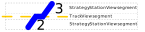
\includegraphics[width=0.9\textwidth]{../img/kap4_trackline_measure_solution}
	\caption{Čáry průběhu jízdy vlaků umístěné do segmentu čar}
	\label{fig:kap4:gttg-model-track-segments-solution}
\end{figure}

Třída \texttt{LinePaint} představuje čáry, které používá například \texttt{TrackView} nebo \texttt{TrainView} k~reprezentaci čar, které, jak jsme si uvedli, můžou měnit svou velikost. \texttt{LinePaint} je \textit{wrapperem} nad \texttt{SKPaint}, které v~knihovně SkiaSharp udává vlastnosti vykreslení čar, textu nebo různých objektů. Vlastnost \texttt{StrokeWidth} třídy \texttt{SKPaint} představuje tloušťku čáry. Třída \texttt{LinePaint} si pamatuje z~konstruktoru přidělenou požadovanou tloušťku čáry \texttt{DesiredStrokeWidth}, kterou poskytuje při měření \texttt{Measure()}. Pomocí \texttt{Arrange()} se pak nastaví jiná tloušťka čáry.

\subsubsection*{Rozšiřující implementace view modelu infrastruktury se strategiemi}
Rozšiřující implementace view modelů podporující strategie s~prefixem \linebreak \texttt{Strategy} v~názvu je potomkem základní implementace view modelů. Tento vztah mezi třídami se nachází na obrázku \ref{fig:kap4:gttg-core-view-model-diagram}. View model infrastruktury se strategiemi rozšiřuje základní implementaci tak, že k~třídám \texttt{RailwayView} a~\texttt{StationView} přidává segmenty v~třídách \texttt{StrategyRailwayView} a~\texttt{StrategyStationView}.

\begin{figure}[!hbt]
	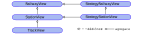
\includegraphics[width=\textwidth]{../img/kap4_gttg-core-view-model-diagram}
	\caption{Závislosti mezi třídami základního view modelu a~rozšiřujícího view modelu se strategiemi}
	\label{fig:kap4:gttg-core-view-model-diagram}
\end{figure}

Na obrázku \ref{fig:kap4:gttg-core-view-model-infrastructure-strategy} se nachází \texttt{MeasureableSegment} segmenty, které zmíněné rozšířené view modely obsahují, kategorizované strukturou \texttt{SegmentType<T>}. \linebreak \texttt{SegmentType<T>} nese informaci o~vizuálním umístění segmentu ve view modelu (\texttt{Lower}, \texttt{Upper}) a~instanci modelu \texttt{T}, kterou je v~těchto view modelech \texttt{Track} nebo \texttt{Station}. \texttt{StrategyRailwayView} obsahují a~určují výšku \texttt{SegmentType<Station>} segmentů, které jsou používány k~umístění čísel vlaků. \texttt{StrategyStationView} obsahují a~určují výšku \texttt{SegmentType<Track>} segmentů, do kterých se umísťují údaje v~ostrých úhlech související s~průběhem jízdy vlaků, jako jsou kóty.

\begin{figure}[!hbt]
	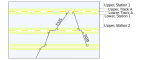
\includegraphics[width=0.9\textwidth]{../img/kap4_gttg-core-view-model-infrastructure-strategy}
	\caption{Zvýrazněné segmenty na nákresném jízdním řádu}
	\label{fig:kap4:gttg-core-view-model-infrastructure-strategy}
\end{figure}
\newpage
\subsubsection*{View model vlaků}
Základní view model vlaků \texttt{Train} je implementován třídou \texttt{TrainView}, která vykresluje šikmou čáru představující průběh jízdy vlaku. Třída pracuje s~typovým  argumentem \texttt{TTrain} odpovídající konkrétní implementaci modelu \texttt{Train}. Jelikož se \texttt{TrainView} nikam na plátně nerozmisťuje, dědí od \texttt{Visual}. Pracuje s~třídou \texttt{TrainPath} jako s implementací \texttt{ITrainPath}, představující šikmou čáru průběhu jízdy vlaku. \texttt{TrainView} obsahuje několik virtuálních metod, jejichž význam si vysvětlíme. Metoda \texttt{UpdateTrainViewContent()} se volá v~případě, když došlo ke změně modelu. Metoda \texttt{Arrange()} se volá v~rámci cyklu rozmístění, kdy se například v~\texttt{TrainPath} musí přepočítat umístění šikmé čáry. Metoda \texttt{OnDraw()} slouží k~vykreslení \texttt{TrainPath} a informací o~vlaku. Nyní si představíme, jak tyto metody modifikují třídu \texttt{TrainPath}.

\subsubsection*{Vykreslení průběhu jízdy vlaku}
\label{kap4:vykresleni_prubehu_jizdy_vlaku}
Třída \texttt{TrainPath} jako součást \texttt{TrainView} spravuje vykreslování šikmé čáry představující průběh jízdy vlaku. Metoda \texttt{Update()} přijímá kolekci \texttt{TrainEvent}, které odpovídají jednotlivým událostem jako odjezd nebo příjezd do stanice. Tyto události pak představují body na čáře průběhu jízdy vlaku, jako na obrázku \ref{fig:kap4:gttg-model-trainPath}.

\begin{figure}[!hbt]
	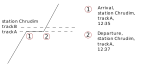
\includegraphics[width=\textwidth]{../img/kap4_train_event_to_train_path}
	\caption{\texttt{TrainEvent} jako body tvořící čáru průběhu jízdy vlaku}
	\label{fig:kap4:gttg-model-trainPath}
\end{figure}

Tloušťka čáry je proměnná a~určuje se při cyklu rozmístění. V~části věnující se \texttt{TrackView} jsme si popsali, že \texttt{TrackView} přidává segmenty do \texttt{SegmentRegistry}, které jsou určeny k~vyměření tlouštěk čar procházející kolejí. \texttt{TrainPath}, představující takovou čáru, získá v~konstruktoru \texttt{SegmentRegistry} a~čáru \texttt{LinePaint}, která se bude vykreslovat a~její tloušťka se bude měnit. V~\texttt{Update()} metodě přidá tuto čáru do segmentů kolejí \texttt{Track} ze všech instancí \texttt{TrainEvent}. 

Metoda \texttt{Update()} se volá v~případě, kdy došlo ke změně průběhu jízdy vlaku. Je možné, že se změní i~koleje \texttt{Track}, kterými vlak projíždí. Proto se v~\texttt{Update()} metodě před provedením zmíněné procedury registrací odstraní původní registrace čar ze všech segmentů.

Metoda \texttt{Arrange()} se volá v~rámci cyklu rozmístění, kdy se musí přerozmístit šikmá čára představující průběh jízdy vlaku. Pomocí rozhraní \texttt{IViewProvider} z~\ref{kap4:graphical_component} se převedou \texttt{DateTime} údaje z~událostí \texttt{TrainEvent} na horizontální souřadnice plátna. Abychom určili vertikální polohu kolejí, získáme ze \texttt{SegmentRegistry} instance segmentů podle instance \texttt{Track} z~každé události. Segmenty obsahují vlastnost \texttt{SegmentContentMiddle}, která určuje umístění středu horizontální čáry koleje na plátně. Z~těchto dvou údajů je sestaven bod \texttt{SKPoint} na čáře, reprezentovanou \texttt{SKPath}. V~metodě \texttt{Draw()} dojde k~vykreslení této čáry použitím \texttt{SKPaint} z~\texttt{LinePaint}.

\subsubsection*{Rozšířený view model vlaků o~strategie}
Třída \texttt{StrategyTrainView} rozšiřuje \texttt{TrainView} o~nástroje, které umožní přidávat k~šikmé čáře vlaku zobrazitelné prvky jako čísla vlaků a~kóty v~ostrých úhlech. Nástroje jsou obsaženy ve \textit{facade} rozhraní \texttt{IStrategy}, jehož konkrétní implementace je vývojáři přístupná jako typový argument \texttt{TStrategy}. Rozhraní obsahuje obecné metody \texttt{Dock()} a~\texttt{Update()} pro práci se strategiemi v~rámci instance \texttt{TrainView}. Metoda \texttt{Dock()}, která rozmístí prvky strategiemi, je volána v~rámci přetížené \texttt{Arrange()} na \texttt{TrainView}. Rozhraní \texttt{IStrategy} implementuje \texttt{IVisual}, čili je vykrelováno v~\texttt{Draw()} metodě a~prvky registrované ve strategiích je možné hit-testovat.

\subsubsection*{Práce se strategiemi pro rozšířený view model infrastruktury}
\label{kap4:strategy}
Rozhraní \texttt{IStrategy} je v~\texttt{GTTG.Model} implementováno třídou \texttt{Strategy}, která je provázána se segmenty view modelu infrastruktury \texttt{StrategyRailwayView} a~\texttt{StrategyStationView}, do kterých umisťuje přidávané prvky. Pro každý \linebreak z~těchto view modelů s~jejich segmenty existuje unikátní strategie. První strategie související se segmenty v~\texttt{SegmentRailwayView} kategorizovaných podle \linebreak\texttt{SegmentType<Station>} slouží k~umisťování čísel vlaků na prostředek čáry mezi dvěma dopravními body, jako na obrázku \ref{fig:kap4:gttg-model-train_number_strategy}.

\begin{figure}[!hbt]
	\centering
	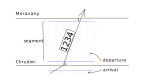
\includegraphics[width=.7\textwidth]{../img/kap4_strategies}
	\caption{Aplikování strategie rozmisťující číslo vlaků mezi dopravní body}
	\label{fig:kap4:gttg-model-train_number_strategy}
\end{figure}

Prvky se do této strategie přidávají přes instanci \texttt{StrategyManager} nazvanou \texttt{StationStrategyManager} uvedením struktury \texttt{TrainEventPlacement}, která prvek umístí ve specifikovaném dopravním bodu \texttt{Station} do horního nebo dolního segmentu, který odpovídá příjezdu nebo odjezdu podle výčtového typu v~třídě \texttt{TrainEvent}, která se do struktury přidává spolu s~výčtovým typem \texttt{AnglePlacement} umísťující prvek do ostrého nebo tupého úhlu. Z~ \texttt{TrainEvent} se pak určí i~instance \texttt{Station}, tvořící \texttt{SegmentType<Station>}. Na následujícím fragmentu kódu přidáváme prvek představující číslo vlaku do tupého úhlu z~události \texttt{TrainEvent}, jejíž typ \texttt{TrainEventType} je odjezd -- \texttt{Departure}. Stejné umístění jako \texttt{Departure} má hodnota průjezdu \texttt{Passage}. Výsledek aplikování zmíněné strategie na umístěný prvek odpovídá obrázku \ref{fig:kap4:gttg-model-train_number_strategy}.

\begin{csharpcode}
var trainNumber = /*.. (ViewElement) ..*/
var trainEvent = /* Station: Chrudim, Type: Departure ...*/
var anglePlacement = AnglePlacement.Obtuse;
var eventPlacement = new TrainEventPlacement(trainEvent, anglePlacement);
strategyManager.Add(eventPlacement, trainNumber);
\end{csharpcode}

Druhá strategie slouží k~umisťování prvků do segmentů kategorizovaných \texttt{SegmentType<Track>} v~\texttt{StrategyTrainView}. Prvky se přidávají do instance \linebreak\texttt{StrategyManager} nazvané \texttt{TrackStrategyManager} uvedením stejné struktury \texttt{TrainEventPlacement} jako pro první strategii. Strategie umisťuje prvky do ostrých nebo tupých úhlů co nejblíže průsečíku šikmé čáry s~horizontální čarou, jako na obrázku \ref{fig:kap4:gttg-model-time_component_strategy}.


\begin{figure}[!hbt]
	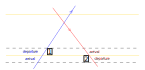
\includegraphics[width=\textwidth]{../img/kap4_segments_track_departure_arrival}
	\caption{Aplikování strategie rozmisťující kóty kolem kolejí}
	\label{fig:kap4:gttg-model-time_component_strategy}
\end{figure}

\newpage
V~metodě \texttt{Dock()} se na přidané prvky z~obou \texttt{StrategyManager} instancí aplikují strategie, které jsou implementací rozhraní \texttt{IStrategyDocker}. V~další části si uvedeme, jak jsou rozhraní pro práci se strategiemi pro tento view model implementovány. 

\subsubsection*{Implementace strategií pro rozšířený view model infrastruktury}
Pro používané strategie v~rámci rozšířeného view modelu \linebreak existují i~implementace rozhraní \texttt{ITypeConverter} a~\texttt{IStrategyDocker}. Třída \texttt{TrainEventPlacementConverter} implementuje rozhraní převodů typu \linebreak \texttt{TrainEventPlacement} do \texttt{SegmentType<Track>} nebo \texttt{SegmentType<Station>}. K~převodům se používá třída \texttt{TrainPath}, čili pro každou instanci \linebreak \texttt{StrategyTrainView} vzniká nový konvertor. Implementace k~převodům používá rozmístění bodů \texttt{TrainPath}, které odpovídají událostem \texttt{TrainEvent}.

Z~typu \texttt{TrainEventPlacement} získáme událost, kterou převedeme. Podle \linebreak směru události \texttt{Departure} nebo \texttt{Arrival} se začne procházet seznam bodů \linebreak v~\texttt{TrainPath}. Nejdříve se najde index odpovídající události. Budeme chtít najít vektor k~jinému bodu v~určeném směru -- pro \texttt{Arrival} hledáme body menších indexů, pro \texttt{Departure} vyšší. Podle vertikálního směru vektoru pak určíme umístění segmentu \texttt{Lower} nebo \texttt{Upper}, jako na obrázku \ref{fig:kap4:gttg-model-time_component_strategy}.

Třídy \texttt{StationStrategyDocker} a~\texttt{TrackStrategyDocker} jako implementace \texttt{IStrategyDocker} pak pomocí tohoto vektoru nachází část cesty představující šikmou čáru ohraničující oblast, kam je prvky možné umístit.%, jako na obrázku \ref{fig:kap4:gttg-model-vector-segment}.

\subsection*{Licence knihovny a~NuGet balíčky}
Celá knihovna GTTG je nabízena pod licencí MIT, více popsané v~souboru \texttt{LICENSE.TXT} umístěném v~kořenovém adresáři příloh práce. Oba dva projekty jsou dostupné jako NuGet balíčky \texttt{GTTG.Core}~\cite{GTTG.Core.NuGet} a~\texttt{GTTG.Model}~\cite{GTTG.Model.NuGet}.